\documentclass[12pt,a4paper]{article}

\usepackage{tikz}
\usetikzlibrary{graphs, graphs.standard, quotes}
\usepackage{tkz-berge}
\usepackage{graphicx}
\usepackage{caption}
\usepackage{tabularx}
\usepackage{algorithmic}
\usepackage{algorithm2e}
\usepackage[utf8]{inputenc}
\usepackage{graphicx}
\usepackage{wrapfig}
\usepackage{float}
\renewcommand{\familydefault}{\rmdefault}


\begin{document}

\begin{titlepage}
	\centering
	\includegraphics[width=0.30\textwidth]{Teclogocompleto.jpg}\par\vspace{1cm}
	{\scshape\large \textbf{Instituto Tecnológico de Costa Rica }\par}
	\vspace{1cm}
	{\scshape\Large MC 6102 Análisis y diseño del Algoritmos\par}
	\vspace{1.5cm}
	{\Large\bfseries Examen I\\Segunda Parte\par}
	\vspace{2cm}
	{\Large\itshape Ricardo Alfaro Villalobos\par}
	\vfill
	Profesor:\par
	Jose Araya Monge\textsc{}

	\vfill

% Bottom of the page
	{\large 30 de setiembre del 2019\par}
\end{titlepage}

\begin{center}
\LARGE \textbf {Apareamiento máximo de aristas}
\end{center}

\begin{section}{Descripción del problema} \noindent 
Dado un grafo $G$ un pareo (matching) de aristas es un subconjunto de las aristas de dicho grafo que cumplen con la condición de ser independientes, es decir, que no tiene un vértice en común\cite{le2014algorithms}.\\\\
Mas formalmente \cite{butenko2003maximum} define un pareo como un conjunto $M$ cuyos elementos son las aristas independientes de un grafo $G=(V,E)$. El problema de $apareamiento\; maximo\; de\; aristas$ consisten en encontrar un pareo con la mayor cardinalidad posible.
\subsection{Cobertura mínima de vértices} \noindent 
Una $cobertura\; de\; vertices\; V'$ es un subconjunto de $V$ tal que cada arista $(i,j) \in E$ tiene al menos un vértice en $V'$. El problema de cobertura mínima de vértices consiste en encontrar una cobertura de vértices con la mínima cardinalidad\cite{butenko2003maximum}.
\subsection{Relación entre estos problemas} \noindent 
El teorema de König relaciona estos dos problemas ya que en el se establece que la cardinalidad un apareamiento máximo de aristas en un grafo bipartito es igual a la cardinalidad de la cobertura mínima de vértices\cite{rizzi2000short}. 
\end{section}

\begin{center}
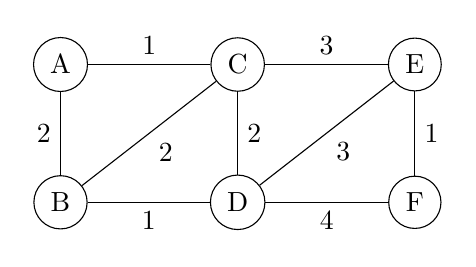
\begin{tikzpicture}[node distance = {1.0cm and 1.5cm}, v/.style = {draw, circle}]
  \graph[nodes={circle, draw}, grow right=2.25cm, branch down=1.75cm]{
    A -- ["1"] C -- ["3"] E,
    B -- ["1",swap] D -- ["4",swap] F,
    B -- ["2"] A,
    C -- ["2"] {D,B},
    D -- ["3",swap] E -- ["1"] F
  };
\end{tikzpicture}
\end{center}

\section{Algoritmos} \noindent 
A continuación se presentan algunos algoritmos para resolver el problema de apareamiento máximo de aristas.

\subsection{Algoritmos voraz}
\begin{algorithmic}
\STATE $i\gets 10$
\IF {$i\geq 5$} 
        \STATE $i\gets i-1$
\ELSE
        \IF {$i\leq 3$}
                \STATE $i\gets i+2$
        \ENDIF
\ENDIF 
\end{algorithmic}
\subsection{Algoritmo Hopcroft–Karp}
\begin{algorithm}[H]
\SetAlgoLined
\KwResult{Write here the result }
 initialization\;
 \While{While condition}{
  instructions\;
  \eIf{condition}{
   instructions1\;
   instructions2\;
   }{
   instructions3\;
  }
 }
 \caption{How to write algorithms}
\end{algorithm}
\section{Aplicaciones} \noindent

\section{Resolver caso} \noindent

\begin{center}
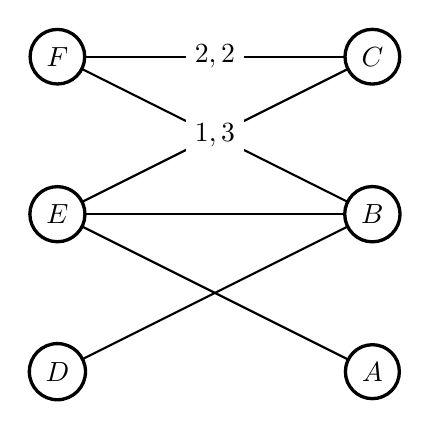
\begin{tikzpicture}[%
  VertexStyle/.style={shape=circle,draw=black,very thick}]
  \Vertex[L=$A$]{a0}          % place a vertex labelled A
  \NO[unit=2,L=$B$](a0){a1}   % place B north of A=a0
  \NO[unit=2,L=$C$](a1){a2}   % place C north of B=a1
  \WE[unit=4,L=$D$](a0){b0}   % place D west of A=a0
  \NO[unit=2,L=$E$](b0){b1}   % place E north of D=b0
  \NO[unit=2,L=$F$](b1){b2}   % place F north of E=b1
  \EdgeFromOneToSel{a}{b}{1}{0}
  \EdgeFromOneToSel{a}{b}{0}{1}
  \EdgeFromOneToSel{a}{b}{1}{1}
  \EdgeFromOneToSel[label={$1,2$}]{a}{b}{1}{2}
  \EdgeFromOneToSel[label={$1,3$}]{a}{b}{2}{1}
  \EdgeFromOneToSel[label={$2,2$}]{a}{b}{2}{2}
\end{tikzpicture}

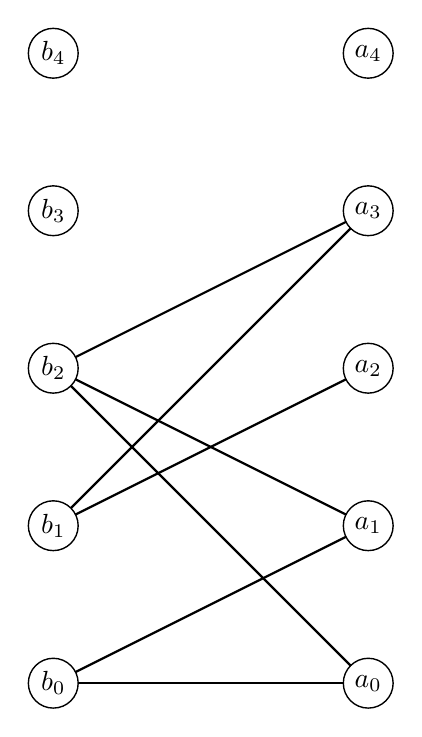
\begin{tikzpicture}
   \begin{scope}[rotate=90]
       \SetVertexMath
       \grEmptyLadder[RA=2,RB=4]{5}   
   \end{scope}
    \Edges(b2,a0,b0,a1,b2,a3,b1,a2)
\end{tikzpicture} 
\hspace{1cm}
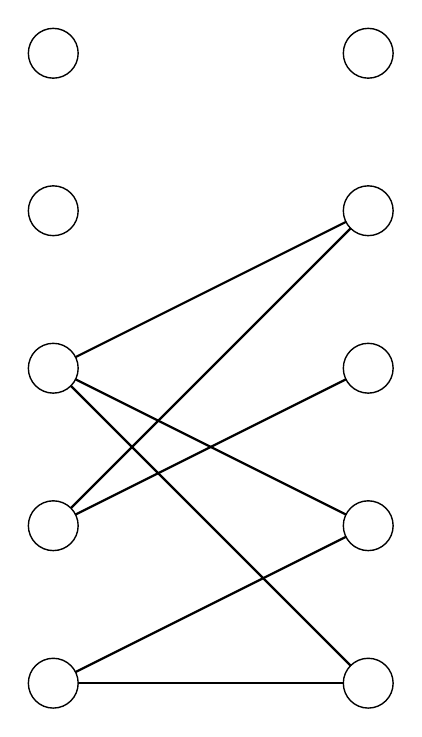
\begin{tikzpicture}
   \begin{scope}[rotate=90]
       \SetVertexNoLabel  
       \grEmptyLadder[RA=2,RB=4]{5}   
   \end{scope}
    \Edges(b2,a0,b0,a1,b2,a3,b1,a2)
\end{tikzpicture} 

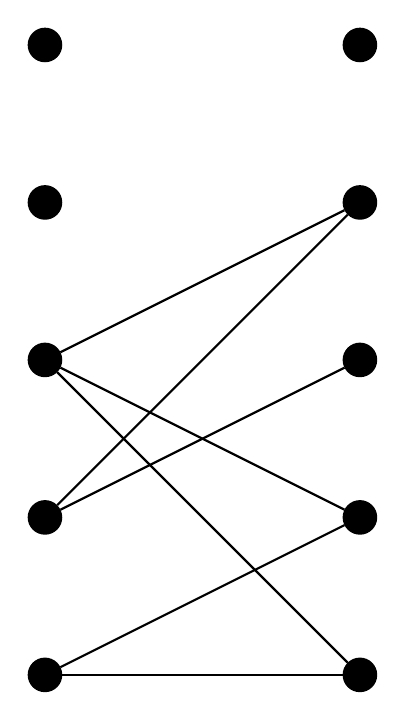
\begin{tikzpicture}
   \begin{scope}[rotate=90]
      \GraphInit[vstyle=Simple]
       \grEmptyLadder[RA=2,RB=4]{5}   
   \end{scope}
    \Edges(b2,a0,b0,a1,b2,a3,b1,a2)
\end{tikzpicture}
\hspace{1cm}
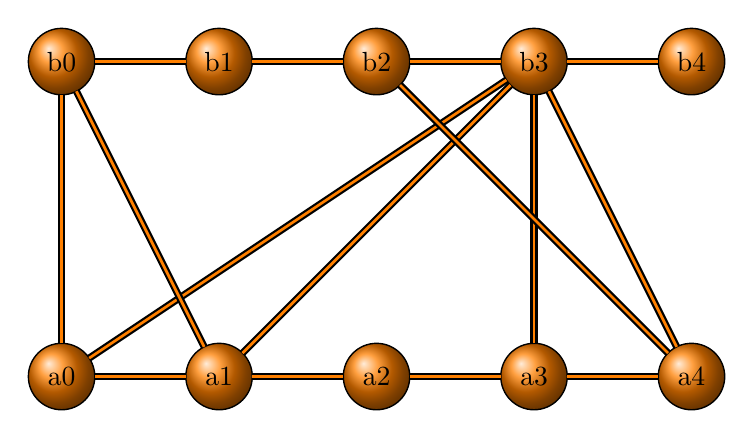
\begin{tikzpicture}
  \GraphInit[vstyle=Shade]
  \grPath[form=1,RA=2]{5}
  \grPath[form=1,prefix=b,RA=2,RS=4]{5}
  \EdgeFromOneToSel{a}{b}{0}{0,3}
  \EdgeFromOneToSel{a}{b}{1}{0,3}
  \EdgeFromOneToSel{a}{b}{3}{3}
  \EdgeFromOneToSel{a}{b}{4}{2,3}    
\end{tikzpicture}
\end{center}
\begin{center}
\begin{figure}[h]
\centering
    \begin{tabularx}{0.8\textwidth}{*{2}{>{\centering\arraybackslash}X}}
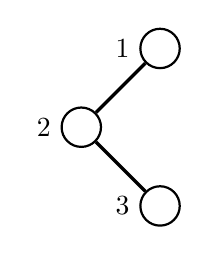
\begin{tikzpicture}[
every edge/.style = {draw=black,very thick},
 vrtx/.style args = {#1/#2}{% 
      circle, draw, thick, fill=white,
      minimum size=5mm, label=#1:#2}
                    ]
\node(A) [vrtx=left/1] at (1, 1) {};
\node(B) [vrtx=left/2] at (0, 0) {};
\node(C) [vrtx=left/3] at (1,-1) {};
%
\path   (A) edge (B)
        (B) edge (C);
\end{tikzpicture}
    \caption*{Figure 1}  
    &   
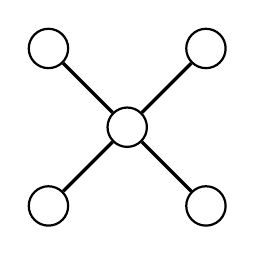
\begin{tikzpicture}[
every edge/.style = {draw=black,very thick},
 vrtx/.style args = {#1/#2}{%
      circle, draw, thick, fill=white,
      minimum size=5mm}
                    ]
\node (A) [vrtx=left/2]     at ( 0, 0) {};
\node (B) [vrtx=left/4]     at (-1, 1) {};
\node (C) [vrtx=right/6]    at ( 1, 1) {};
\node (D) [vrtx=right/8]    at ( 1,-1) {};
\node (E) [vrtx=left/10]    at (-1,-1) {};
 %
\path   (A) edge (B)
        (A) edge (C)
        (A) edge (D)
        (A) edge (E);
\end{tikzpicture}
\caption*{Figure 2}  
    \end{tabularx}
\end{figure}
\end{center}

\newpage
\nocite{*}
\bibliographystyle{ieeetr}
\bibliography{bibliography/ref}
\end{document}
